\chapter{Desarrollo software del manipulador}
\label{cap:capitulo6}

\vspace{1cm}
\noindent En este capítulo se aborda el desarrollo software necesario para poder usar el robot realizado 
tanto en simulaciones como en el mundo real.

\section{Control de los actuadores}
\noindent En esta sección se concretan los mecanismos y herramientas software utilizadas para poder controlar, desde 
un ordenador cualquiera, el hardware creado en el anterior capítulo.

\subsection{Grbl como \textit{firmware} del robot}
\noindent Para realizar el control de los actuadores se ha tomado la decisión de utilizar el 
firmware de control numérico Grbl\ref{subsec:grbl}, por encima 
de realizar uno propio, debido a que es una solución robusta con años de desarrollo y con unas ciertas garantías dificiles de superar.
\\
Actualmente, este firmware permite controlar hasta 3 motores paso a paso simultáneamente. Además, tiene la posibilidad de utilizar 
un canal PWM (usualmente usado en las CNC para modificar la velocidad de la herramienta). Sobre estos motores, podemos realizar 
un control en posición, es decir, recibe una serie de coordenadas y automáticamente alcanza esos puntos. Este tipo de controlador 
es perfectamente válido para esta aplicación y simplifica bastante su uso. Aunque esta placa en concreto viene con Grbl 1.1 instalado 
de fábrica, existen numerosas guías en Internet acerca de como instalarlo.

Para que Grbl sepa qué posición debe tener cada motor en un momento dado, necesita recibir 
una serie de datos codificados a través de una de sus interfaces. Los detalles esta la comunicación 
se presentan en la siguiente subsección.
\newpage
\subsection{Comunicación con Grbl}
\noindent En esta sección se exponen las distintas opciones de comunicación con el robot, así como el formato de mensaje que se debe emplear.
\\ 
\indent Debido a las características hardware de la placa utilizada, se puede establecer comunicación con Grbl a través de 2 interfaces diferentes. 
La primera, es a través del propio puerto USB integrado, utilizando el protocolo serie UART. Este modo de comunicación tiene la ventaja de 
ser rápido pero te fuerza a estar conectado al robot a través de un cable. Por otro lado, debido a las características técnicas del 
microcontrolador, se puede establecer una comunicación inalámbrica a través de Wifi utilizando el protocolo Telnet. Finalmente, se ha optado 
por utilizar la interfaz USB debido a que es más rápida y permite al usuario estar conectado a internet, en vez de a la propia red 
\textit{offline} que crea la placa.

\indent Una forma de poder saber si viene ya instalado en la placa que hemos comprado, es utilizar una terminal serie, como 
puede ser \textit{Cutecom}. Establecemos una velocidad de 115200 baudios y nos conectamos al puerto que aparezca disponible 
al conectar la placa al ordenador. Si está instalado, veremos una serie de mensajes que indican la versión de Grbl y las 
distintas configuraciones internas. (Figura \ref{fig:cutecom})
\begin{figure} [ht!]
\begin{center}
    \includegraphics[width=14cm]{figs/cutecom.png}
\end{center}
\caption{Terminal gráfica de Cutecom al conectarse a una placa con Grbl}
\label{fig:cutecom}
\end{figure}

\indent Grbl recibe instrucciones de G-Code\ref{sec:gcode} a través del puerto serie. Aunque existen una gran 
cantidad de ellas, solo ha sido necesario usar algunas:
\begin{table}[H]
\begin{center}
\begin{tabular}{|l|l|}
\hline
\textbf{Comando} & \textbf{Explicación} \\
\hline
G92 X0 Y0 Z0 & G92 establece los valores de posición de cada eje\\
G01 & Establece que todos los ejes se moverán a la vez de forma lineal  \\
G90 X1 Y2 Z3 F34 & Mueve los motores a velocidad 34 hasta una coordenada absoluta  \\
S500 & Establece la velocidad del motor auxiliar a 500. Rango: 0-1000  \\
M3 & Enciende el motor auxiliar  \\
M5 & Apaga el motor auxiliar  \\
? & Pecibir el estado actual de la maquina  \\
! & Para el movimiento actual \\
\textasciitilde & Continua con el movimiento parado anteriormente \\
\hline
\end{tabular}
\caption{Comandos utilizados en la realización del proyecto}
\end{center}
\end{table}


Con el objetivo de abstraer al futuro software del robot de esta comunicación, se ha implementado 
una clase en Python\ref{subsec:pyhton} llamada \textit{Grbl}. En este software, utiliza la librería 
PySerial\footnote{\url{https://pypi.org/project/pyserial/}} para establecer una comunicación serie.

\noindent La clase \textit{Grbl} creada puede ser utilizada a través de los siguientes métodos:

\begin{lstlisting}[language=Python,  literate={á}{{\'a}}1 {é}{{\'e}}1 {í}{{\'i}}1 {ó}{{\'o}}1 {ú}{{\'u}}1 {ñ}{{\~n}}1]
start(puerto) # Devuelve true/false en función de si ha sido posible conectarse
stop() # Finaliza la comunicación
setSpindleSpeed(value) # Establece la velocidad del motor auxiliar
enableSpindle() # Activa el motor auxiliar
disableSpindle() # Desactiva el motor auxiliar
setCoordinates(x, y, z) # Establece las coordenadas x, y, z 
getXYZ() # Devuelve la posición actual
asyncXYZMove(posición, velocidad, relative) # Mueve los motores a una posición con la velodicad dada. Permite realizar movimientos relativos y absolutos.
\end{lstlisting}

Su código fuente puede ser encontrado en el repositorio del 
proyecto\footnote{\url{https://github.com/RoboticsURJC/tfg-vperez/blob/96fc1e44bef6a31c272fb0673b5a33a7571c5ee7/src/software/g_arm/g_arm/g_arm_lib/grblAPI.py}}.
\\

A pesar de que ya podemos comandar movimientos en los distintos ejes de la máquina, se requiere realizar una serie 
de configuraciones para definir las características concretas de cada articulación.
\newpage
\subsection{Configuración de Grbl para su uso en robótica}
\noindent GRBL tiene ciertas limitaciones a la hora de usarse en robótica. Es normal, debido a que está pensado para controlar máquinas 
\acs{CNC} de 3 ejes prismáticos. Pese a esto, se pueden unas ciertas configuraciones para adaptarlo a esta aplicación. 

\subsubsection{Parámetros de Grbl}
Este \textit{firmware} guarda en su memoria interna una serie de parámetros que definen su 
comportamiento. Si se quiere visualizar cuáles son y sus respectivos valores, hay que enviar 
el mensaje \textbf{\$\$} a través del puerto serie. Para modificar un cierto valor, hay que introducir una cadena 
con el formato: \textbf{\$identificador del parámetro=nuevoValor}.

Para modificar la configuración de una forma cómoda, se recomienda utilizar herramientas como 
\textit{UniversalGcodeSender} (Figura \ref{fig:ugs}).

\begin{figure} [ht!]
\begin{center}
    \includegraphics[width=15cm]{figs/ugs.png}
\end{center}
\caption{Interfaz de UniversalGcodeSender\footnote{\url{https://winder.github.io/ugs_website/download/}}}
\label{fig:ugs}
\end{figure}

Puesto que se quiere utilizar Grbl para controlar un brazo robot, debemos 
realizar las siguientes configuraciones:
\begin{itemize}
\item \textbf{\$1}: Retardo o tiempo de espera entre pulsos de paso cuando el motor está inactivo (en milisegundos). 
\\Debemos configurar 
este parámetro en su valor máximo, en este caso 255. Este valor tiene un significado especial, haciendo que los motores paso a paso 
se mantengan energizados constantemente aunque no se estén moviendo. Es de vital importancia para evitar que el brazo se desplome al detenerse en una cierta posición.  
\item \textbf{\$100}, \textbf{\$101} y \textbf{\$102}: Indican el número de pasos por unidad de movimiento para los ejes X, Y, Z respectivamente. 
\\Por defecto está pensado para utilizar pasos por milímetro. Como se pretende utilizar articulaciones de rotación, debemos expresar esta relación 
en función de alguna medida angular. La unidad a utilizar podría ser: grados, radianes o vueltas, entre otras. En este trabajo se 
utilizan los grados debido a que en radianes y vueltas la unidad correspondía a un gran número de pasos y era dificil controlar la aceleración para incrementos de 
0.1 vueltas. 

\begin{myequation}[h!]
\begin{equation}
    PasosPorGrado = \frac{Microstepping * Ratio}{1.8^\circ}
\nonumber
\label{ec:pasos_por_grado}
\end{equation}
\caption[Cálculo de pasos por grado en Grbl]{Cálculo de pasos por grado en Grbl}
\end{myequation} 

\item \textbf{\$110}, \textbf{\$111} y \textbf{\$112}: Indican la velocida máxima a la que puede moverse cada eje X, Y, Z en unidades por segundo. 
En este caso, grados por segundo. Estos valores se deben encontrar por medio de la experimentación. Se trata de una medida de seguridad en 
caso de que el usuario quiera mover demasiado rápido un eje pudiendo dañar el brazo.

\item \textbf{\$120}, \textbf{\$121} y \textbf{\$122}: Indican la aceleración máxima a la que puede moverse cada eje X, Y, Z en unidades por segundo cuadrado. 
En este caso, grados por segundo cuadrado. Estos valores tambien se deben encontrar por medio de la experimentación. Se trata de una medida de seguridad en 
caso de que el usuario quiera mover demasiado rápido un eje pudiendo dañar el brazo. Se debe encontrar una aceleración idónea para todos 
los movimientos, una limitación de grbl es que no se puede comandar un movimiento diciendole una determinada aceleración.
\end{itemize}

Para profundizar más en la finalidad de cada parámetro, código y configuración se 
recomienda leer la documentación \footnote{\url{https://github.com/gnea/grbl/blob/master/doc/markdown/commands.md}}
\footnote{\url{https://github.com/gnea/grbl/blob/master/doc/markdown/settings.md}}
\\
\newpage
En el caso concreto de este proyecto, se ha utilizado la configuración mostrada en la Tabla \ref{cuadro:parametros_grbl}.
\\

\begin{table}[H]
\begin{center}
\begin{tabular}{|c|c|}
\hline
\textbf{Parámetro} & \textbf{Valor} \\
\hline
\textdollar0 & $10$ \quad (Step pulse time, microseconds) \\
\textdollar1 & $255$ \quad (Step idle delay, milliseconds) \\
\textdollar2 & $0$ \quad (Step pulse invert, mask) \\
\textdollar3 & $1$ \quad (Step direction invert, mask) \\
\textdollar4 & $0$ \quad (Invert step enable pin, boolean) \\
\textdollar5 & $1$ \quad (Invert limit pins, boolean) \\
\textdollar6 & $1$ \quad (Invert probe pin, boolean) \\
\textdollar10 & $1$ \quad (Status report options, mask) \\
\textdollar11 & $0.010$ \quad (Junction deviation, millimeters) \\
\textdollar12 & $0.002$ \quad (Arc tolerance, millimeters) \\
\textdollar13 & $0$ \quad (Report in inches, boolean) \\
\textdollar20 & $0$ \quad (Soft limits enable, boolean) \\
\textdollar21 & $0$ \quad (Hard limits enable, boolean) \\
\textdollar22 & $1$ \quad (Homing cycle enable, boolean) \\
\textdollar23 & $1$ \quad (Homing direction invert, mask) \\
\textdollar24 & $1.000$ \quad (Homing locate feed rate, mm/min) \\
\textdollar25 & $1.000$ \quad (Homing search seek rate, mm/min) \\
\textdollar26 & $250.000$ \quad (Homing switch debounce delay, milliseconds) \\
\textdollar27 & $1.000$ \quad (Homing switch pull-off distance, millimeters) \\
\textdollar30 & $10000.000$ \quad (Maximum spindle speed, RPM) \\
\textdollar31 & $0.000$ \quad (Minimum spindle speed, RPM) \\
\textdollar32 & $0$ \quad (Laser-mode enable, boolean) \\
\textdollar100 & $26.666$ \quad (X-axis travel resolution, step/mm) \\
\textdollar101 & $22.222$ \quad (Y-axis travel resolution, step/mm) \\
\textdollar102 & $22.222$ \quad (Z-axis travel resolution, step/mm) \\
\textdollar110 & $6000.000$ \quad (X-axis maximum rate, mm/min) \\
\textdollar111 & $6000.000$ \quad (Y-axis maximum rate, mm/min) \\
\textdollar112 & $6000.000$ \quad (Z-axis maximum rate, mm/min) \\
\textdollar120 & $60.000$ \quad (X-axis acceleration, mm/sec\textasciicircum2) \\
\textdollar121 & $60.000$ \quad (Y-axis acceleration, mm/sec\textasciicircum2) \\
\textdollar122 & $60.000$ \quad (Z-axis acceleration, mm/sec\textasciicircum2) \\
\textdollar130 & $450.000$ \quad (X-axis maximum travel, millimeters) \\
\textdollar131 & $450.000$ \quad (Y-axis maximum travel, millimeters) \\
\textdollar132 & $50.000$ \quad (Z-axis maximum travel, millimeters) \\
\end{tabular}
\caption{Parámetros Grbl usados en este trabajo}
\label{cuadro:parametros_grbl}
\end{center}
\end{table}

\newpage
\section{Integración con ROS 2}
\noindent En esta sección se detalla el proceso de integración del robot G-Arm en \acs{ROS}, pasando 
por la creación de la descripción, la visualización, la configuración y la simulación. 

\subsection{Descripción del robot}
\noindent El primer paso en la integración de un robot en el ecosistema ROS, es lograr expresar 
su forma y funcionamiento de tal manera que pueda ser visualizado, simulado y controlado en el mundo 
virtual. Esto es conocido como describir un robot y para ello existen diferentes formatos entre los que destacan URDF y Xacro.

\subsubsection{Creación del paquete de descripción}
\noindent Para crear el paquete, se ha seguido el siguiente
\begin{enumerate}
    \item En el \textit{src} del workspace ejecutamos:
    \begin{verbatim}
        ros2 pkg create --build-type ament_cmake g_arm_description
    \end{verbatim}   
    \item Dentro de la carpeta que se ha generado, creamos 3 nuevos directorios:
    \begin{verbatim}
        mkdir launch rviz urdf meshes
    \end{verbatim} 
        
    \item Añadimos al fichero \textit{package.xml}: 
    \lstset{
        language=XML, % Establece el lenguaje como XML
        basicstyle=\ttfamily, % Fuente monoespaciada
        keywordstyle=\bfseries\color{blue}, % Estilo de las palabras clave
        commentstyle=\itshape\color{gray}, % Estilo de los comentarios
        stringstyle=\color{orange}, % Estilo de las cadenas de texto
        showstringspaces=false, % No mostrar espacios en cadenas de texto
        breaklines=true, % Dividir líneas largas
        frame=lines, % Agregar un marco alrededor del código
        numbers=left, % Mostrar números de línea
        numberstyle=\tiny\color{gray}, % Estilo de los números de línea
        captionpos=b % Posición de la leyenda del código (abajo)
    }
    
    \begin{lstlisting}
        <exec_depend>joint_state_publisher</exec_depend>
        <exec_depend>robot_state_publisher</exec_depend>
        <exec_depend>rviz</exec_depend>
        <exec_depend>xacro</exec_depend>
    \end{lstlisting}
    
    \item Compilamos el paquete desde la raíz del workspace:
    \begin{verbatim}
        colcon build --symlink-install
    \end{verbatim}
    \item Añadimos la siguiente línea al final del .bashrc para que ROS pueda encontrar el paquete:
    \begin{verbatim}
        source ~/workspace/install/local_setup.bash
    \end{verbatim}
    
    \end{enumerate}

\subsubsection{Describir un robot mediante URDF y Xacro}
\ac{URDF} es un formato de archivo cuyo propósito es describir la estructura, cinemática y aspecto de un robot.  
Se trata de un estándar ampliamente utilizado en la comunidad robótica, especialmente en \ac{ROS}.

En este tipo de archivo, se especifica la geometría del robot mediante la definición de eslabones (links) 
y articulaciones (joints). 
Cada eslabón es descrito por su aspecto y geometría, mientras que las articulaciones están definidas
en cuanto a su tipo, recorrido y posición. Además de esto, un archivo URDF puede incluir información 
sobre la masa y la inercia de los eslabones, así como como texturas y modelos 3D.

\begin{figure} [ht!]
    \begin{center}
        \includegraphics[width=10cm]{figs/urdf.png}
    \end{center}
    \caption{Elementos del formato URDF\footnote{\url{http://library.isr.ist.utl.pt/docs/roswiki/urdf\%282f\%29XML\%282f\%29Joint.html}}}
\label{fig:urdf}
\end{figure}
Este formato se basa en el lenguaje \ac{XML}, lo que permite describir el robot de una forma 
estructurada y legible. Por otro lado, Xacro es un lenguaje de macros XML que simplifica la 
creación de descripciones URDF al permitir la reutilización de código y la parametrización 
de modelos. Se puede convertir un fichero Xacro a URDF ejecutando el siguiente comando:
\begin{verbatim}
    xacro fichero.xacro > fichero.urdf
\end{verbatim}
\newpage
Con el objetivo de lograr una descripción lo más realista posible, se han empleado las mismas geometrías del diseño \acs{CAD}.
Para poder incluirlas en el URDF, es necesario exportar las piezas al formato \textit{Collada} (.dae) desde FreeCAD. Este formato 
contiene información acerca de la geometría, posición, tamaño y colores, de la pieza en cuestión.
\\
Además del aspecto visual, hay que definir el volumen físico que ocupan en el espacio. Las mallas de colisión son la representación 
geométrica simplificada utilizada para calcular interacciones físicas y detectar colisiones en simulaciones. En este caso se va a utilizar 
un formato muy liviano de malla, el \ac{STL}. 

Tanto los ficheros Collada como los ficheros STL, deben estar en la carpeta \textit{meshes} creada anteriormente. En cambio; el fichero 
URDF debe estar en la carpeta \textit{urdf}.
\\

Un aspecto a tener en cuenta, es que no todos los tipos de robot pueden ser descritos con este formato. La limitación radica en que 
un eslabón hijo solo soporta un eslabón padre, por lo que no se pueden construir cadenas cinemáticas cerradas. \\
\begin{figure} [ht!]
    \centering  
    \subfigure[Cerrada]{\label{fig:abierta}\includegraphics[width=0.3\linewidth ]{figs/cerrada.png}}
    \hspace{2cm}
    \subfigure[Abierta]{\label{fig:cerrada}\includegraphics[width=0.3\linewidth ]{figs/abierta.png}}
    \caption{Cadenas cinemáticas}
  \end{figure}\ 
\\
El robot de este trabajo esta constituido enteramente por cadenas cinemáticas cerradas. Pese a esto, se ha utilizado el ingenio y un tipo de 
articulación específico para lograr describir este tipo de robot de forma exacta. Se llama \textit{Mimic joint} y
es un tipo de articulación pasiva que imita el ángulo de otra. Con una cierta combinación de varias de ellas, y una serie de 
eslabones invisibles se puede lograr describir este tipo de robot. 
Además, ha sido necesario añadir una cuarta articulación \enquote{falsa}. Esta indica la intensidad del electroimán acoplado al robot. 
Es de tipo revolución, pero su recorrido es de 0.001 radianes por lo que apenas afecta a la cinemática. 

El fichero\footnote{\url{https://github.com/RoboticsURJC/tfg-vperez/blob/8d3b281d701ec4a57602a9dcfcdd04888955319b/src/software/g_arm_description/urdf/robot_electromagnet.urdf}} 
URDF final puede ser encontrado junto al resto del proyecto en el repositorio de Git.
\newpage
\subsubsection{Creación de un launcher para visualizar el robot}
\noindent Para visualizar el fichero que hemos creado anteriormente, podemos realizar una herramienta de ROS 
llamada RViz. Esta herramienta no solo permite visualizar, sino también analizar datos de sensores, modelos de robot y 
planificaciones de movimiento de forma interactiva. Además se le pueden añadir complementos para agregale funcionalidades extra. 
\\

Para que se pueda cargar la descripción del robot en este visualizador, debe haber algo que la esté publicando en el topic 
\textit{robot\_description}. Es por esto que existe un nodo de ROS llamado \textit{robot\_state\_publisher} que se encarga 
de ello. Además, si queremos algo más que una representación estática, podemos utilizar un nodo llamado \mbox{\textit{joint\_state\_publisher\_gui}}. Este nodo 
muestra una ventana gráfica con una serie de controles para controlar manualmente cada joint. 
\\

Teniendo en cuenta que se requiere lanzar una serie de nodos y programas, es útil crear un \textit{launcher} de ROS. Un \textit{launcher} es una 
herramienta que se utiliza para iniciar, configurar, gestionar y desplegar nodos. Este tipo de fichero terminado en 
\textit{.launch.py} se almacenan en la carpeta \textit{launch}. Para crearlo, se ha usado como inspiración el lanzador \textit{visualize\_franka.launch.py} del 
robot Franka Emika\footnote{\url{https://github.com/frankaemika/franka_ros2/blob/develop/franka_description/launch/visualize_franka.launch.py}}.
\\

Finalmente, el paqute de descripción está terminado. Ejecutando el siguiente comando, se nos abrirá una ventana de RViz y una 
serie de controles deslizantes para cada articulación (Figura \ref{fig:rviz}).
\begin{verbatim}
    ros2 launch g_arm_description display_tool.launch.py
\end{verbatim}

\begin{figure} [ht!]
    \begin{center}
        \includegraphics[width=15cm]{figs/RViz.png}
    \end{center}
    \caption{Ventana de RViz visualizado el robot creado}
\label{fig:rviz}
\end{figure}

\newpage
\subsection{Integración con MoveIt 2}
\noindent En esta sección se enumeran y describen los pasos necesarios para, apartir de un paquete de descripción de un robot, generar 
un paquete de MoveIt.
\\
Antes de comenzar, debemos tener instalado MoveIt 2 para ROS Humble. Para ello, se ha seguido el proceso de 
instalación\footnote{\url{https://moveit.picknik.ai/main/doc/tutorials/getting_started/getting_started.html}} de la documentación.
\\

Para crear el paquete de MoveIt de este robot, se han llevado a cabo los siguientes pasos:
\begin{enumerate}
\item Lanzamos el asistente de configuración.
\begin{verbatim}
    ros2 launch moveit_setup_assistant setup_assistant.launch.py
\end{verbatim}
\item Pulsamos sobre \textbf{\textit{\guillemotleft Create New MoveIt Configuration Package\guillemotright}} y cargamos el URDF/Xacro del paquete de descripción 
del robot. Si el fichero es válido, aparecerán una serie de apartados a configuar en el lateral izquierdo del asistente. 
\item Comenzamos configurando la apartado \textbf{\textit{\guillemotleft Self-Collisions\guillemotright}}. Aquí se hace uso de la colisiones 
descritas anteriormente para generar una matriz de posibles colisiones que se pueden dar. Para ello, pulsamos sobre
\textbf{\textit{\guillemotleft Generate Collision Matrix\guillemotright}}.
\item Acto seguido se configura el apartado \textbf{\textit{\guillemotleft Planning Groups\guillemotright}}, donde se establecen los eslabones y articulaciones que serán consideradas 
a la hora de realizar la planificación. Para ello, pulsamos sobre \textbf{\textit{\guillemotleft Add Group\guillemotright}} y acto seguido 
le damos un nombre. Posteriormente, pulsamos sobre \textbf{\textit{\guillemotleft Add Kin. Chain\guillemotright}} y seleccionamos como 
eslabón base, el eslabón que irá unido al suelo, y como eslabón \textit{tip}, el extremo del robot (sin llegar a la herramienta). Entonces, guardamos los cambios. Ahora, 
se añaden todos los \textit{links} y \textit{joints} de la cadena anterior, al grupo de planificación creado, dando en \textbf{\textit{\guillemotleft Edit Selected\guillemotright}}.
Repetimos este procedimiento con el grupo de planificación de la herramienta, seleccionando como eslabón base el eslabón final de la anterior cadena, y como 
final de esta, el último eslabón de la herramienta. 

\item En el apartado \textbf{\textit{\guillemotleft Robot Poses\guillemotright}} se pueden configurar una serie de posiciones predeterminadas 
para poder usarse posteriormente cuando se necesiten. Por ejemplo, es recomendable crear al menos dos; una que haga de posición \textit{Home} 
(Posición cómoda para empezar a trabajar) y otra como posición de reposo (Posición que evita que el robot se desplome al cortar la electricidad). Además 
podemos añadir dos más para el grupo de planificación de la herramienta: \textit{ToolON} y \textit{ToolOFF}.

\item Usamos el apartado \textbf{\textit{\guillemotleft End Effectors \guillemotright}} para configurar el extremo de nuestro robot como tal. Para ello, 
seleccionamos el eslabón del extremo y el grupo de planificación creado anteriormente. 

\item En \textbf{\textit{\guillemotleft Passive Joints\guillemotright}}, añadimos todos aquellas articulaciones que no sean grados de libertad, 
es decir, todas aquellas que no sean \textit{joint1, joint2, joint3, jointPWM (señal PWM de la herramienta)}.

\item En los apartados \textbf{\textit{\guillemotleft ROS 2 Controllers\guillemotright}} y 
\textbf{\textit{\guillemotleft MoveIt Controllers\guillemotright}}, añadimos automaticamente los controladores pulsando sobre el único botón que hay.

\item Finalmente rellenamos nuestra información personal en \textbf{\textit{\guillemotleft Author information\guillemotright}} y generamos el 
paquete en el \textit{src} del \textit{workspace}. Acto seguido, compilamos.
\end{enumerate}

A la hora de usar esta herramienta, se debe de tener en cuenta que a día de la publicación de este trabajo, existe un error en el asistente
que hace que el paquete no se cree bien del todo. Para corregirlo, es necesario cambiar todos los número del fichero \textit{joints\_limits.yaml}
del paquete generado a \textit{double}. Es decir, cambiar por ejemplo un ``200" por ``200.0".
\\
\newpage
Para comprobar que el paquete ha sido configurado bien, ejecutamos un \textit{launcher} generado automáticamente por el asistente :
\begin{verbatim}
    ros2 launch g_arm_moveit demo.launch.py
\end{verbatim}
Tras ejecutarlo, se debería abrir una ventana de RViz con un aspecto similar a lo mostrado en la Figura \ref{fig:moveit_demo}. Podemos utilizar 
el propio \textit{plugin} de MoveIt para establecer una posición aleatoria y tratar de llegar a ella (Figura \ref{fig:moveit_trayectory_demo}).
\begin{figure} [ht!]
    \begin{center}
      \includegraphics[width=13cm]{figs/moveit_demo.png}
    \end{center}
    \caption{Rviz al lanzar el \textit{demo.launch.py}}
    \label{fig:moveit_demo}
\end{figure}\ 

\begin{figure} [ht!]
    \begin{center}
      \includegraphics[width=13cm]{figs/moveit_demo_trajectory.png}
    \end{center}
    \caption{Planificando una trayectoria simple}
    \label{fig:moveit_trayectory_demo}
\end{figure}\ 

\subsection{Driver para ROS}
\noindent En esta sección se detalla el funcionamiento del nodo ROS creado para ejecutar las trayectorias en el robot real.
\\


Primeramente es necesario comprender el funcionamiento de este framework, al menos su parte más externa, aquella que 
se comunica con el exterior. 
Según la documentación\footnote{\url{https://moveit.picknik.ai/humble/doc/concepts/move_group.html}}, existe 
un nodo llamado \textit{move\_group} (Véase la Figura\ref{fig:arquitectura_moveit}) que se comunica con resto del framework 
a través de los topics y acciones de ROS. De cara al exterior, puede establecer conexión con dos elementos del propio entorno del robot. 
El primero es la percepción, en este caso permite obtener información de la escena a través de los datos de una cámara 3D. El segundo es el 
controlador del robot, que se encarga de aceptar y ejecutar las trayectorias requeridas, además de devolver información acerca del 
progreso.
\begin{figure} [ht!]
    \begin{center}
      \includegraphics[width=12cm]{figs/moveit_arquitectura.png}
    \end{center}
    \caption{Relación de \textit{move\_group} con el resto del \textit{Firmware}}
    \label{fig:arquitectura_moveit}
\end{figure}\ 
\newpage
Según la propia documentación, la forma más simple y eficaz de controlar el robot real es utilizando un controlador de 
\mbox{\textit{ros2\_control}\footnote{\url{https://control.ros.org/master/index.html}}}
e imitar en el robot real las posiciones de los distintos joints publicadas por el controlador. En sí \mbox{\textit{ros2\_control}} es un 
framework que incorpora una gran cantidad de herramientas para implementar sistemas de control en ROS. Dentro de él, existen los llamados 
controladores y según su tipo pueden controlar robots de tracción diferencial, direcciones Ackermann, entre otros. Para esta aplicación el que nos 
interesa es \mbox{\textit{Joint Trajectory Controller}}, un controlador diseñado para ejecutar trayectorias en el espacio de 
articulaciones, interpolando entre uno o más puntos de referencia. Conjuntamente con esto, hay que 
utilizar otro nodo llamado \textit{joint\_state\_broadcaster}, que lee las interfaces de estado del controlador y las publica en los topics
\textit{/dynamic\_joint\_states} y \textit{/joint\_states}. Siendo finalmente este último topic el que deberá ser escuchado por el 
nodo del robot real para extraer la posición 
de cada articulación. En el Bloque de código \ref{cod:campos} se muestran los campos del mensaje enviado a través 
de él.
\lstset{language=C++,
        basicstyle=\ttfamily,
        keywordstyle=\color{blue},
        commentstyle=\color{green},
        stringstyle=\color{orange},
        showstringspaces=false,
        breaklines=true,
        breakatwhitespace=true}

\begin{code}[h]
\begin{lstlisting}
Header header

string[] name
float64[] position
float64[] velocity
float64[] effort
\end{lstlisting}
\caption{Campos del tipo de mensaje \mbox{\textit{sensor\_msgs/msg/JointState}}}
\label{cod:campos}
\end{code}

El driver creado, hace uso de una clase intermedia entre el nodo ROS y la clase \textit{grbl} con el fin de abstraer al nodo de la conversión 
de unidades. Además, esta nueva clase incorpora lo necesario para encontrar los límites físicos de cada articulación sumado a una serie de 
constantes usadas para hacer que la posición absoluta de las articulaciones concuerde con la usada en la descripción del robot. \\

Al comenzar, trata 
de conectarse al robot y busca el 0,0 de cada joint. Posteriormente crea una subscripción al topic \textit{/joint\_states} para recibir y 
guardar el último mensaje que llega a través de  este topic. En paralelo a esto, existe una función llamada con una cierta frecuencia (utilizando un 
\textit{timer} de ROS) que envía las posiciones del mensaje, previamente guardado, al robot real. Se ha decidido separar ambos comportamientos 
para tener un cierto control sobre la frecuencia de envíos de datos por el puerto serie y evitar saturar el firmware del robot. 
\newpage
En la Figura \ref{fig:dia_driver1} se muestra el diagrama de actividades que ilustra el funcionamiento básico del driver creado.\\
\\


\begin{figure} [ht!]
    \begin{center}
      \includegraphics[width=12cm]{figs/driver_diagram1.jpg}
    \end{center}
    \caption{Diagrama de actividades del driver}
    \label{fig:dia_driver1}
\end{figure}\ 


Por suerte, el propio lanzador de demostración mencionado en la sección anterior, ya levanta estos nodos por lo que no es necesario crear 
uno nuevo para realizar las pruebas. Más adelante sí es recomendable hacerlo, para poder tener mayor control sobre los nodos 
que se están lanzando y añadir nuevos si es necesario.
\\

\newpage
\section{Pruebas}
\noindent En esta sección se ponen a prueba los aspectos técnicos que determinan el desempeño y la fiabilidad del brazo robot. Para ello, 
se han llevado a cabo una serie de tests, bajo distintas circunstancias, y se han apuntado los resultados.
características.

\subsection{Estabilidad y flexión}
\noindent En esta prueba se determina afectan diferentes fuerzas a la estructura del propio brazo, evaluando por ejemplo, cuanto se dobla 
cuando se le aplica una cierta carga.
Para ello, se han considerado los siguientes 3 escenarios:
\begin{itemize}
    \item Escenario 1: El robot está completamente retraido y se le aplican una serie de cargas de 10 a 150 gramos.
    \item Escenario 2: El robot está en una posición de operación normal y se le aplican una serie de cargas de 10 a 150 gramos.
    \item Escenario 3: El robot está completamente extendido horizontalmente y se le aplican una serie de cargas de 10 a 150 gramos.
\end{itemize}

\begin{figure} [ht!]
    \centering
    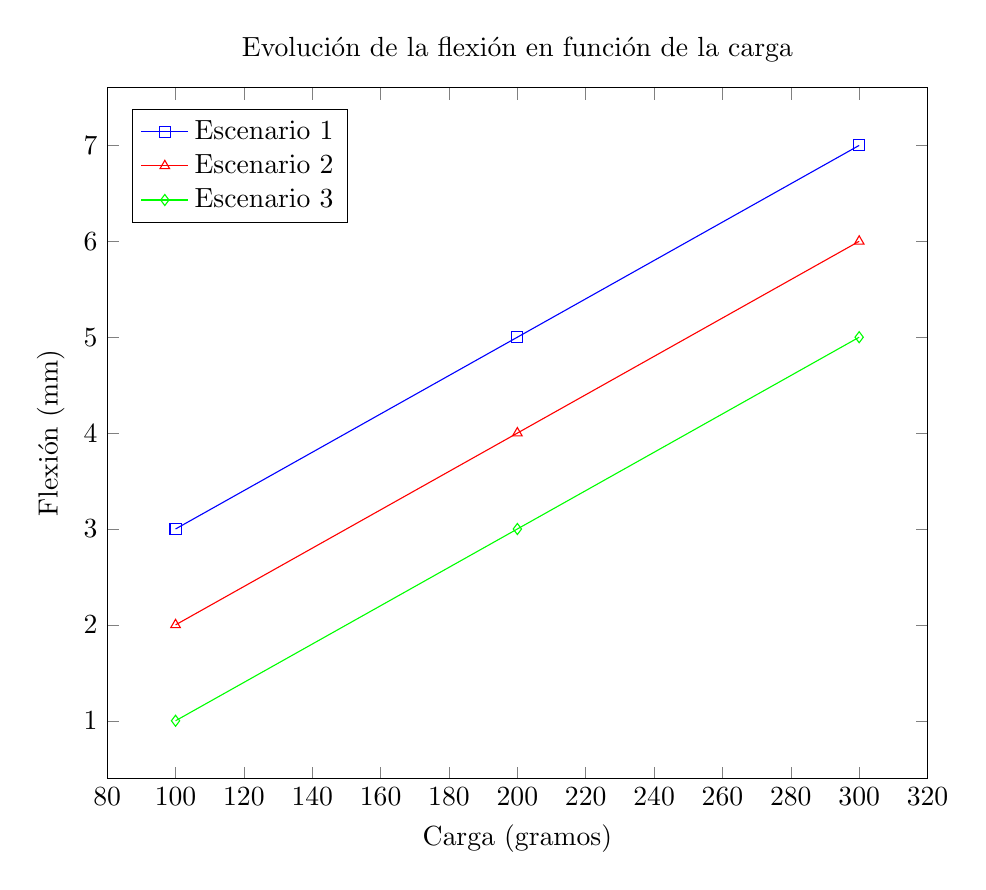
\begin{tikzpicture}
      \begin{axis}[
        width=12cm, 
        %height=8cm,  
        xlabel={Carga (gramos)},
        ylabel={Flexión (mm)},
        legend pos=north west, % Posición de la leyenda
        title={Evolución de la flexión en función de la carga}
      ]

      % Datos de los tres escenarios
      \addplot [color=blue, mark=square] coordinates {
        (100, 3)
        (200, 5)
        (300, 7)
        % ...
      };
      
      \addplot [color=red, mark=triangle] coordinates {
        (100, 2)
        (200, 4)
        (300, 6)
        % ...
      };
      
      \addplot [color=green, mark=diamond] coordinates {
        (100, 1)
        (200, 3)
        (300, 5)
        % ...
      };
      
      % Leyendas para las series de datos
      \legend{Escenario 1, Escenario 2, Escenario 3}
      
      \end{axis}
    \end{tikzpicture}
    \caption{Gráfica de evolución de flexión en función de la carga aplicada}
    \label{fig:grafica-flexion}
  \end{figure}
En cuanto a la estabilidad, el robot es capaz de mantenerse en su posición más extendida de forma horizontal si volcar hasta los 400g 
de peso. Esto considerando que la base no está anclada al suelo de ninguna manera. Aún así, a la hora de hacer movimientos en los que involucra 
la rotación de la base, la propia inercia hace que, al frenar y acelerar, la base se deslice. Por lo que es recomendable atornillar la base al 
suelo o ponerle unas patas de goma antideslizante. 

\subsection{Capacidad de carga}
\noindent En este apartado se pone a prueba la capacidad del robot a la hora de levantar y mover cargas con diferentes masas. Concretamente, 
se realiza esta prueba para encontrar las limitaciones a la hora de manipular objetos pesados. \\
En esta prueba se han considerado los siguientes escenarios:
\begin{itemize}
    \item Escenario 1: El robot comienza a nivel de suelo, con el extremo del robot lejos de la base y empieza a levantar lentamente las distintas cargas. La 
    prueba finaliza cuando los motores empiezan a perder pasos y no son capaces de elevar la carga.
    \item Escenario 2: Repetir el escenario 1 pero situando la carga cerca de la base del robot.
    \item Escenario 3: El robot hace uso de su herramienta electroimán (teóricamente de 3Kg de fuerza) para levantar distintas cargas unidas a un 
    objeto ferromagnético. La prueba finaliza cuando el electroimán no es capaz de sujetar la carga o bien, el robot no es capaz de levantarla.
\end{itemize}
\begin{table}[H]
\begin{center}
\begin{tabular}{|c|c|}
\hline
\textbf{Escenario} & \textbf{Carga máxima} \\
\hline
Escenario 1& \SI{10}{\kilo\gram} \\
Escenario 2 & \SI{10}{\gram} \\
Escenario 3 & \SI{10}{\gram} \\
\hline
\end{tabular}
\caption{Resultados de los diferentes resultados en la prueba de carga}
\label{cuadro:evaluacion_carga}
\end{center}
\end{table}
\newpage
\subsection{Velocidad y tiempo de respuesta}
\noindent En esta prueba se evalúa que tan rápido se puede mover sin afectar a su funcionamiento normal 
llevando diferentes cargas. Además, se determina que tan rápido se responde a una orden desde la capa 
de nivel de ROS, hasta el propio movimiento.

\begin{table}[H]
\begin{center}
\begin{tabular}{|c|c|}
\hline
\textbf{Parámetro} & \textbf{Valor} \\
\hline
Velocidad máxima & \SI{10}{\meter\per\second}\\
Aceleración máxima & \SI{10}{\meter\per\second}\\
Tiempo de respuesta (señal de la herramienta) & \SI{35}{\milli\second} \\
Tiempo de respuesta (movimiento del brazo) & \SI{35}{\milli\second} \\
\hline
\end{tabular}
\caption{Evaluación de la velocidad y tiempo de respuesta}
\label{cuadro:evaluacion_velocidad}
\end{center}
\end{table}

\subsection{Exactitud y repetitividad} 
Se procede a realiza pruebas para evaluar la precisión del brazo robot en la ejecución de movimientos y la repetibilidad 
de estos movimientos. Se mide la desviación del brazo robot en comparación con las coordenadas objetivo y verificar si 
es capaz de alcanzar de manera consistente los mismos puntos en un cierto número de intentos.

\subsection{Consumo eléctrico} 
\label{sec:consumo}
\noindent Este tipo de pruebas evaluan cuanta energía está consumiendo el robot bajo unas conciciones concretas. Es útil para 
conocer el coste de tener en funcionamiento este robot y si es viable utilizarlo sobre plataformas móviles a baterías. 
\\
Para realizar este test, se han considerado 4 escenarios:
\begin{itemize}
\item Escenario 1: El robot se mueve sin ningún tipo de carga realizando un movimiento rápido entre dos puntos alejados.
\item Escenario 2: El robot se mueve sin ningún tipo de carga realizando un movimiento lento entre dos puntos alejados.
\item Escenario 3: El robot se mueve con una carga de 50g gramos (mando a distancia de la televisión) a velocidad moderada entre dos puntos alejados.
\item Escenario 4: El robot se mueve con una carga de 100 gramos (teléfono móvil) a velocidad moderada entre dos puntos alejados.

\end{itemize}
Los resultados de las pruebas se muestran en el Cuadro \label{cuadro:consumos}.
\begin{table}[H]
\begin{center}
\begin{tabular}{|c|c|c|}
\hline
\textbf{Escenario} & \textbf{Consumo medio} & \textbf{Pico de consumo}\\
\hline
Escenario 1 & \SI{10}{\meter\per\second} & w\\
Escenario 2 & \SI{10}{\meter\per\second} & 2\\
Escenario 3 & \SI{35}{\milli\second} & s \\
Escenario 4 & \SI{35}{\milli\second} & df\\
\hline
\end{tabular}
\caption{Consumos eléctricos en distintos escenarios}
\label{cuadro:consumos}
\end{center}
\end{table}